%Time-stamp: "Last modified: 2018-08-02 10:42:16 (d_yasaki)"
\documentclass[ms]{uncgdissertationexp}
\setcounter{secnumdepth}{1}
% default is 12pt, phd, doublespaced.
% Masters students should use the ma on as shown below.
% \documentclass[ma]{uncgdissertation}

%%------------------------------------------------------------------%%
%%------------------------- Import Packages ------------------------%%
%%------------------------------------------------------------------%%
%% This is where you can put other packages that you may need.
\usepackage[lofdepth,lotdepth,caption=false]{subfig}
\usepackage{fancyhdr}
\usepackage{amsmath, amssymb, graphicx}
\usepackage{xspace}
\usepackage{braket}
\usepackage{color}
\usepackage{setspace}
\usepackage{fancyvrb}
\usepackage{array}
\usepackage{ifxetex,ifluatex}
\usepackage{etoolbox}
\usepackage{booktabs}
\usepackage{xcolor}
\usepackage{tabu}
\usepackage{longtable}
\usepackage{titlesec}
\usepackage{lmodern}

\usepackage{microtype, amsfonts, amsthm}
\usepackage[colorlinks=false]{hyperref}
\pdfstringdefDisableCommands{\let\MakeUppercase\relax}
%\usepackage{showframe}
%useful package to ensure margins are correct.

% fix for pandoc 1.14
\providecommand{\tightlist}{
  \setlength{\itemsep}{0pt}\setlength{\parskip}{0pt}}

\def\tightlist{} 
%%tightlist error

%%I don't know what this does...
%\usepackage{color}
\usepackage{fancyvrb}
\newcommand{\VerbBar}{|}
\newcommand{\VERB}{\Verb[commandchars=\\\{\}]}
\DefineVerbatimEnvironment{Highlighting}{Verbatim}{commandchars=\\\{\}}
% Add ',fontsize=\small' for more characters per line
\usepackage{framed}
\definecolor{shadecolor}{RGB}{248,248,248}
\newenvironment{Shaded}{\begin{snugshade}}{\end{snugshade}}
\newcommand{\KeywordTok}[1]{\textcolor[rgb]{0.13,0.29,0.53}{\textbf{#1}}}
\newcommand{\DataTypeTok}[1]{\textcolor[rgb]{0.13,0.29,0.53}{#1}}
\newcommand{\DecValTok}[1]{\textcolor[rgb]{0.00,0.00,0.81}{#1}}
\newcommand{\BaseNTok}[1]{\textcolor[rgb]{0.00,0.00,0.81}{#1}}
\newcommand{\FloatTok}[1]{\textcolor[rgb]{0.00,0.00,0.81}{#1}}
\newcommand{\ConstantTok}[1]{\textcolor[rgb]{0.00,0.00,0.00}{#1}}
\newcommand{\CharTok}[1]{\textcolor[rgb]{0.31,0.60,0.02}{#1}}
\newcommand{\SpecialCharTok}[1]{\textcolor[rgb]{0.00,0.00,0.00}{#1}}
\newcommand{\StringTok}[1]{\textcolor[rgb]{0.31,0.60,0.02}{#1}}
\newcommand{\VerbatimStringTok}[1]{\textcolor[rgb]{0.31,0.60,0.02}{#1}}
\newcommand{\SpecialStringTok}[1]{\textcolor[rgb]{0.31,0.60,0.02}{#1}}
\newcommand{\ImportTok}[1]{#1}
\newcommand{\CommentTok}[1]{\textcolor[rgb]{0.56,0.35,0.01}{\textit{#1}}}
\newcommand{\DocumentationTok}[1]{\textcolor[rgb]{0.56,0.35,0.01}{\textbf{\textit{#1}}}}
\newcommand{\AnnotationTok}[1]{\textcolor[rgb]{0.56,0.35,0.01}{\textbf{\textit{#1}}}}
\newcommand{\CommentVarTok}[1]{\textcolor[rgb]{0.56,0.35,0.01}{\textbf{\textit{#1}}}}
\newcommand{\OtherTok}[1]{\textcolor[rgb]{0.56,0.35,0.01}{#1}}
\newcommand{\FunctionTok}[1]{\textcolor[rgb]{0.00,0.00,0.00}{#1}}
\newcommand{\VariableTok}[1]{\textcolor[rgb]{0.00,0.00,0.00}{#1}}
\newcommand{\ControlFlowTok}[1]{\textcolor[rgb]{0.13,0.29,0.53}{\textbf{#1}}}
\newcommand{\OperatorTok}[1]{\textcolor[rgb]{0.81,0.36,0.00}{\textbf{#1}}}
\newcommand{\BuiltInTok}[1]{#1}
\newcommand{\ExtensionTok}[1]{#1}
\newcommand{\PreprocessorTok}[1]{\textcolor[rgb]{0.56,0.35,0.01}{\textit{#1}}}
\newcommand{\AttributeTok}[1]{\textcolor[rgb]{0.77,0.63,0.00}{#1}}
\newcommand{\RegionMarkerTok}[1]{#1}
\newcommand{\InformationTok}[1]{\textcolor[rgb]{0.56,0.35,0.01}{\textbf{\textit{#1}}}}
\newcommand{\WarningTok}[1]{\textcolor[rgb]{0.56,0.35,0.01}{\textbf{\textit{#1}}}}
\newcommand{\AlertTok}[1]{\textcolor[rgb]{0.94,0.16,0.16}{#1}}
\newcommand{\ErrorTok}[1]{\textcolor[rgb]{0.64,0.00,0.00}{\textbf{#1}}}
\newcommand{\NormalTok}[1]{#1}
%
% commands and environments needed by pandoc snippets
% extracted from the output of `pandoc -s`
%% Make R markdown code chunks work

\ifxetex
  \usepackage{fontspec,xltxtra,xunicode}
  \defaultfontfeatures{Mapping=tex-text,Scale=MatchLowercase}
\else
  \ifluatex
    \usepackage{fontspec}
    \defaultfontfeatures{Mapping=tex-text,Scale=MatchLowercase}
  \else
    \usepackage[utf8]{inputenc}
  \fi
\fi
\DefineShortVerb[commandchars=\\\{\}]{\|}
\DefineVerbatimEnvironment{Highlighting}{Verbatim}{commandchars=\\\{\}}
% Add ',fontsize=\small' for more characters per line



%%------------------------------------------------------------------%%
%%--------------------------- Content ------------------------------%%
%%------------------------------------------------------------------%%
%% Members of committee.  Guidelines say don't use Dr.
%% Masters students are required to have chair plus two
%% PhD students require chair plus three.
%% The class can handle up to chair plus five.
\chair{Parke Rublee}
\member{Anne Hershey}
\member{Martin Tsui}
%%\member{}

%% Your name goes here.
%% \student{Firstname}{Lastname}
%% Some other options
%%\student{Joe Michael}{Schmoe}  % a full middle name
\student{Ashley S.}{Williams}       % a middle initial

%% Thesis Title
%%    +  Capitalize first letter of important words.
%%    +  Use inverted pyramid shape if title spans more than one line.
%%  Note: You can force break the title onto multiple lines using
%%  \break instead of \\.
\title{Response of Mercury Methylating Bacteria to the Dan River Coal Ash Spill
with a Survey of Metal Tolerance of Microorganisms Associated with Coal
Ash}

%% Degree year.
\degreeyear{2019}


%%------------------------------------------------------------------%%
%%----------------------- Personal Macros --------------------------%%
%%------------------------------------------------------------------%%
%% A central location to add your favorite macros.  A few examples are
%% given below.  See tips for samples.

%% In order to get singlespacing, uncomment the line below.
%\renewcommand{\doublespacing}{\singlespacing}

%% Theorem, Lemma, etc. environments.  You can rename if you wish.
% Theorem style and numbering convention
\theoremstyle{plain}
\newtheorem{theorem}{Theorem}[chapter]
\newtheorem{lemma}[theorem]{Lemma}
\newtheorem{proposition}[theorem]{Proposition}
\newtheorem{conjecture}[theorem]{Conjecture}
\newtheorem{corollary}[theorem]{Corollary}
\newtheorem{algorithm}[theorem]{Algorithm}

% Definition type object style and numbering convention
\theoremstyle{definition}
\newtheorem{definition}[theorem]{Definition}
\newtheorem{example}[theorem]{Example}

% Remark type object style and numbering
\theoremstyle{remark}
\newtheorem*{remark}{Remark}  % the star makes them not numbered
\newtheorem*{notation}{Notation}
\newcommand{\titlecaption}[2]{\caption[#1]{#1. #2}}

%% Other macros
\newcommand{\ZZ}{\mathbb{Z}}  % Integers
\newcommand{\XX}{\mathfrak{X}}

%\bibliography{references}

%%------------------------------------------------------------------%%
\begin{document}
\frontmatter      % required

%%------------------------------------------------------------------%%
%% -------------------------- Abstract -----------------------------%%
%%------------------------------------------------------------------%%
\begin{abstract}
  This is my abstract. The abstract page is a required component of the
  thesis/dissertation. The abstract should be a brief summary of the
  paper, stating only the problem, procedures used, and the most
  significant results and conclusions. Explanations and opinions are
  omitted. Remember to include the necessary information regarding any
  multimedia components included in the document. The abstract must be
  approved by your advisor/committee chair.
\end{abstract}
%%------------------------------------------------------------------%%
%%---------------------------- Title page --------------------------%%
%%------------------------------------------------------------------%%
%% The title page is required.
\maketitlepage

%%------------------------------------------------------------------%%
%% ------------------------ Copyright page -------------------------%%
%%------------------------------------------------------------------%%
%% This page is required if you opt for a copyright.  Otherwise, don't
% include it.  To omit, just comment out the line below.
%\makecopyrightpage

%%------------------------------------------------------------------%%
%%---------------------------- Dedication --------------------------%%
%%------------------------------------------------------------------%%
\begin{dedication}
  The dedication is often short. Longer statements are usually in the
  acknowledgements. The dedication is optional.
\end{dedication}
%%------------------------------------------------------------------%%
%%------------------------ Approval page  --------------------------%%
%%------------------------------------------------------------------%%
%% The approval page is required.  If all of your infomation is entered
%% correctly in the contents section, this should come out correctly.
\makeapprovalpage

%%------------------------------------------------------------------%%
%%-------------------------- Acknowledgements ----------------------%%
%%------------------------------------------------------------------%%
%% The acknowledgements are optional but highly recommended.  See tips
%% for details.
\begin{acknowledgments}
  It is customary to recognize the assistance of the advisor and/or
  committee chair, all other members of the committee, and only those
  organizations and/or persons who actually aided the research. If
  financial support was provided to make the study possible, credit for
  such assistance should be given.
\end{acknowledgments}
%%------------------------------------------------------------------%%
%%----------------------------- Preface ----------------------------%%
%%------------------------------------------------------------------%%
%% The preface is optional.
%%\begin{preface}
%%A preface is a statement that either explains the author's
%%reasons for pursuing this subject matter or provides a personal
%%comment about the subject that would not otherwise be included in
%%the document.
%%\end{preface}


%%------------------------------------------------------------------%%
%%---------------------- Table of Contents -------------------------%%
%%------------------------------------------------------------------%%
%% The table of contents is required.
\tableofcontents

%%------------------------------------------------------------------%%
%%---------------------- List of Tables ----------------------------%%
%%------------------------------------------------------------------%%
% Recommended if you have tables.  Comment out if you don't have
% tables.

  \listoftables
  

%%------------------------------------------------------------------%%
%%---------------------- List of Figures ---------------------------%%
%%------------------------------------------------------------------%%
% Recommended if you have figures.  Comment out if you don't have
% figures.

  \listoffigures
  

%%------------------------------------------------------------------%%
%% This signifies that you are done with the frontmatter and ready to
%% proceed to the main part.  The rest of your document goes below.
\mainmatter % required
%%------------------------------------------------------------------%%
 
  \chapter{Introduction}\label{intro}
  
  Coal is the second most used fuel for electricity generation in the
  United States. In 2017, approximately 30\% of all electricity production
  was fueled by coal combustion (Administration, 2019). Although the
  percentage has fallen in recent years due to retirement of plants and
  increase in natural gas and other energy sources, coal remains a main
  fuel for electricity. During the process of coal combustion, coal
  combustion residuals, or coal ash, is produced.
  
  Coal combustion residues (CCRs) include fly ash, bottom ash, and flue
  gas desulfurized gypsum. Fly ash is a fine powdery substance, comprised
  primarily of silica that moves up the exhaust system. It is produced
  during the combustion of finely ground coal and most is captured from
  the exhaust using electrostatics and scrubber systems (US EPA, 2014a).
  Bottom ash is formed during the combustion of pulverized coal in
  boilers. It ranges in size from fine sand to fine gravel and is grey to
  black in color. Bottom ash is too large to be carried up the exhaust
  system and is collected in an ash hopper (US EPA, 2014b). Flue gas
  desulfurized gypsum is not a direct product of coal combustion, but a
  product of the scrubber system to remove SO2 emissions from exhaust (US
  EPA, 2014c).
  
  Physical and chemical properties of coal ash are determined by the
  geographical location where the raw coal was mined, the type of boiler,
  and the operating conditions of the power plant (Jayaranjan et al.,
  2014). Fly ash is composed mainly of oxides such as \(\mathrm{SiO_2}\),
  \(\mathrm{Al_2O}\), \(\mathrm{Fe_2O}\), \(\mathrm{TiO_2}\), and
  \(\mathrm{CaO}\). All natural elements can be found in coal ash, trace
  elements include, As, Cd, Cr, Hg, Pb, Se, and Zn (Greely Jr. et al.,
  2014; Jayaranjan et al., 2014; Shaheen et al., 2014). Coal bottom ash
  consists of silicate, carbonate, aluminate, ferrous materials and
  several of heavy metals and metalloids. Like fly ash, the chemical
  composition of the bottom ash is dependent on the source of the raw
  coal, boiler type, and the refinement process of the raw coal
  (Jayaranjan et al., 2014).
  
  Once produced and collected, CCRs are transported to an impoundment pond
  or landfill. Impoundment ponds are constructed either lined or unlined;
  open to the atmosphere or capped. In an open lagoon, the waste settles
  to the bottom of the pond, leaving the shallow surface water free of
  waste. To prevent overflow of these ponds, this shallow water is pumped
  and directed to a waterway adjacent to the power plant. In the US, of
  the approximately 120 Mt of CCRs are produced annually, 54\% is disposed
  of in landfills or surface impoundments (American Coal Ash Association,
  2012). Leaching and impoundment failures allow the mobilization of CCRs
  including their associated heavy metals into the environment, where
  these metals may enter the food web directly or indirectly through
  microbially-mediated transformations (Cabral et al., 2016; Deonarine et
  al., 2013; Otter et al., 2012).
  
  \chapter{RESPONSE OF MERCURY METHYLATING BACTERIA TO THE COAL ASH SPILL
  IN THE DAN RIVER}\label{pcr}
  
  \section{Abstract}\label{abstract}
  
  \section{Introduction}\label{introduction}
  
  On February, 2, 2014, two storm water drainage pipes located under a
  coal ash impoundment pond at the Duke Energy Dan River Steam Station
  near Eden, NC collapsed, releasing approximately 28,000 cubic yards of
  coal ash and about 27 million gallons of untreated ash wastewater into
  the Dan River (Dennis Lemly, 2015). Following the spill, water and
  sediment was sampled from the river and Kerr Reservoir downstream of the
  spill to determine water quality and human health concerns. Test results
  show no constituents to be at levels exceeding safe limits in the water
  column (US EPA, 2014d). Duke Energy dredged ash deposits at two
  locations along the river, but likely over 90\% of the ash remains
  buried in river sediments or has been deposited into Kerr Lake (NC DEQ,
  2014). While the test results are encouraging for immediate water
  quality, the long-term concern is the effect of mobilization of coal ash
  constituents into the riverine food webs.
  
  One constituent of particular concern during leaching and/or impoundment
  failure is mercury. Mercury, a known neurotoxin and potential endocrine
  disruptor has a high affinity for sulfhydryl groups in proteins where
  destabilization leads to decreased enzymatic activity and reduced
  overall fitness (Driscoll et al., 2013; Ehrlich and Newman, 2008). In
  submerged anoxic sediments under certain conditions, inorganic mercury
  (\(\mathrm{Hg^{2+}}\)) can be converted into MeHg by microbial
  metabolism (Dash and Das, 2014; Schaefer et al., 2011). Methylmercury
  (MeHg) bioaccumulates and biomagnifies in the river food webs, posing a
  health risk to local residents who consume fish. (Dash and Das, 2014;
  Otter et al., 2012; Rowe, 2014). The total available amount of MeHg
  within an ecosystem is controlled by multiple microbial and abiotic
  processes that reduce availability of \(\mathrm{Hg^{2+}}\) or
  degradation of MeHg. \(\mathrm{Hg^{2+}}\) can be volatilized as
  \(\mathrm{Hg^{0}}\) through photoreduction or by bacteria with the merA
  gene (Boyd and Barkay, 2012). Additionally, MeHg can be demethylated
  into \(\mathrm{Hg^{2+}}\) by sunlight (Tsui et al., 2013) or microbes
  with the merB gene (Bizily et al., 1999).
  
  Microorganisms have developed various mechanisms to mitigate effects of
  high concentrations of heavy metal toxins. These include reduction of
  the metal to a less toxic form, metal complexation, efflux pumps via an
  energy-dependent membrane transporter, and extracellular sequestration
  (Binkley and Simpson, 2003; Poulain and Barkay, 2013). MeHg is produced
  in anaerobic conditions predominately by sulfate reducing bacteria (SRB)
  iron reducing bacteria (IRB) and methanogens (Liu et al., 2014). Coal
  ash may provide the necessary substrates such as sulfates to stimulate
  the microbial methylation of Hg (Deonarine et al., 2013).
  
  Two genes are required for methylation of Hg, hgcA and hgcB. As
  \(\mathrm{Hg^{2+}}\) enters the cell, a methylated-HgcA protein
  transfers a CH3 group to \(\mathrm{Hg^{2+}}\) within the cytosol. HgcB
  protein is then required to recycle the methylated-HgcA protein (Poulain
  and Barkay, 2013). The hgcAB sequence is conserved across multiple
  genera and therefore could be utilized as a molecular biomarker for
  suspected contaminated sites with real-time quantitative PCR
  (Christensen et al., 2016; Dash and Das, 2014; Lima de Silva et al.,
  2012; Parks et al., 2009). Liu et al. (2014) found that the hgcA
  abundance and the concentration of MeHg in rice paddy soil near the
  Wanshan Hg mining area was positively correlated (Liu et al., 2014).
  This finding suggests that microbes may be contributing to the MeHg in
  the sampled soils. They also found high genetic diversity within the
  microbial community and that environmental factors such as total Hg,
  \(\mathrm{SO_4}\), \(\mathrm{NH_4}\), and organic matter influenced the
  community structure. After phylogenetic analysis, the representative
  taxa in the community consisted of Deltaproteobacteria, Firmicutes,
  Chloroflexi, Euryarchaeota, and two novel taxa (Liu et al., 2014).
  
  In 2008 a dike failure at the Tennessee Valley Authority Kingston Fossil
  Plant coal ash pond in Harriman, Tennessee, released an estimated 5.4
  million cubic yards of ash into the surrounding community and rivers
  (Ruhl et al., 2010). The release ruptured a natural gas line, disrupted
  power and transportation, destroyed three homes, and resulted in the
  evacuation of nearby neighborhoods. The impoundment pond has since been
  rebuilt and reinforced to resist natural disasters such as earthquakes
  (TVA, 2011). In sediment samples collected downstream following the
  spill, total mercury concentrations were three to four times greater
  than sediments upstream of the spill. MeHg was also slightly higher than
  upstream (Deonarine et al., 2013).
  
  The coal ash spill into the Dan River has mobilized heavy metals into
  the environment. The extent of long-term effects of methylated mercury
  into the food chain in the river is unknown. Mercury, along with other
  coal ash constituents may stimulate mercury-methylating microorganisms
  in anaerobic sediments. The goal of this study is to determine the
  overall microbial community response and specifically hgcA abundance as
  a result of the Dan River coal ash spill.
  
  \subsection{Objective and hypothesis:}\label{objective-and-hypothesis}
  
  Determine spatial distribution of mercury-methylating taxa as a result
  of the coal ash spill using qPCR. I hypothesize that there will be
  increased abundance of the hgcA genes and therefore, mercury methylating
  taxa downstream of spill site due to stimulation of sulfate and iron
  reducing bacteria and methanogens by coal ash constituents present in
  the sediment.
  
  \section{Methods}\label{methods}
  
  \subsection{Study Sites and Sediment
  Collection}\label{study-sites-and-sediment-collection}
  
  The Dan River is a 344 km river that rises in Patrick Co. Virginia and
  crosses into North Carolina in Stokes County. It flows across the border
  between NC and VA several times before flowing into the Kerr Reservoir
  on the Roanoke River which then flows to the Atlantic Ocean at the
  Albemarle Sound in North Carolina. This study encompasses sites upstream
  of the spill site in Eden, NC and downstream to Milton, NC, a 103 km
  section of the Dan.
  
  To characterize the extent of the coal ash spill impact on the microbial
  community, samples were collected at three upstream reference sites, one
  site parallel to the ash ponds but upstream of the spill (leaching
  site), and five downstream sites including near two sites that were
  dredged for remediation, one at Town Creek, near the spill site and one
  near Abreu-Grogan Park, Danville, Va., and depositional sites that were
  not dredged near Danville (Figure \ref{fig:map}).
  \begin{Shaded}
  \begin{Highlighting}[]
  \NormalTok{knitr}\OperatorTok{::}\KeywordTok{include_graphics}\NormalTok{(}\DataTypeTok{path =} \StringTok{"figure/map.png"}\NormalTok{)}
  \end{Highlighting}
  \end{Shaded}
  \begin{figure}
  
  {\centering 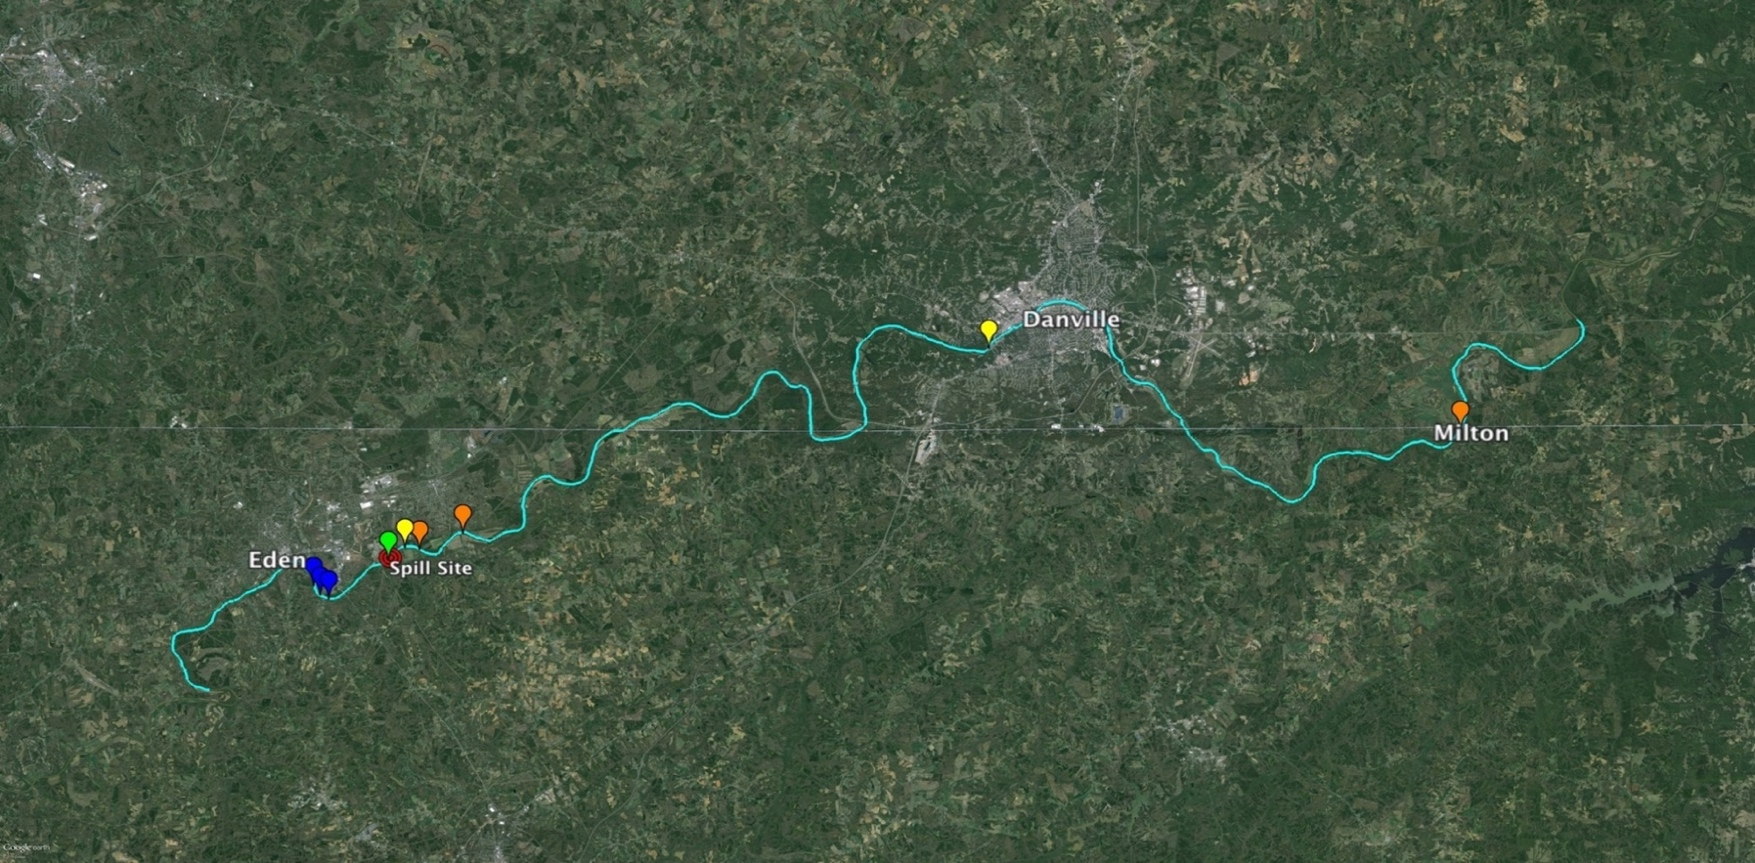
\includegraphics[width=400pt]{figure/map} 
  
  }
  
  \caption{Map}\label{fig:map}
  \end{figure}
  Each site was accessed by motorboat, where sediment from the riverbank
  and channel was collected. Riverbank sediment cores were collected in
  triplicate using a piston-stule coring device. Channel samples were
  collected using a small dredge. Sediment cores were segmented by depth
  and mixed according to one of three sampling schemes to reduce the total
  number of samples to be assayed. 0.25 \(\mathrm{cm^3}\) samples were
  preserved in CTAB (cetyltrimethylammonium bromide) for DNA extraction.
  Channel sediment was mixed thoroughly then 0.25 \(\mathrm{cm^3}\) was
  preserved in CTAB.
  
  Sampling Scheme:
  \begin{enumerate}
  \def\labelenumi{\Alph{enumi}.}
  \item
    Sediment cores extracted in triplicate, each 0-8 cm and 8-16 cm
    segments sampled
  \item
    Triplicate sediment cores pooled at 0-2 cm, 10-12 cm, 15-17 cm
  \item
    Triplicate sediment cores pooled 0-8 cm and 8-16 cm segments sampled.
  \end{enumerate}
  \subsection{DNA extraction and qPCR}\label{dna-extraction-and-qpcr}
  
  A CTAB extraction was performed using standard protocol for each sample
  (Stewart and Via 1993). The DNA extracted was quantified and
  subsequently diluted to a standard concentration of 5 ng/L and stored in
  a 4C refrigerator. Extracted DNA quantity and purity were determined
  from 2 μl subsamples of each extraction using Thermo Scientific Nanodrop
  Spectrophotometer based on the 260/280 wavelength ratio.
  
  An Applied Biosystems StepOne\^{}TM real-time PCR System was utilized to
  detect, amplify, and quantify target DNA gene proxies and representative
  taxa to meet the Objective. Primers were chosen from the literature
  based on targeting a general metabolic category. These include generic
  primers to the hgcA gene, a sulfate reducing gene, dsr, the 16S rDNA of
  iron reducing bacteria, and methanogens (Geets et al. 2008, Schaefer et
  al. 2013, Wagner et al.1998, Wright and Primm 2003, Table X). This
  approach will define the microbial community abundance encompassed
  within each sample. Each reaction contained the following: 10µL of Power
  Sybr® Green PCR master mix, 1µL of forward primer, 1µL of reverse
  primer, 8µL of sterile deionized water, and 1µL of extracted DNA. Three
  negative control reactions, samples repeated in triplicate, and positive
  standard controls serially diluted in triplicate, were ran in each 48
  well plate. The relative abundance of targets were computed by the
  StepOne software using the generated standard curve. The melt curve was
  examined to manually ensure that none of the amplifications were due to
  a false positive. Statistical analyses including one and two-way ANOVA
  and regression analyses were performed to determine if a significant
  difference exists between amounts of targeted DNA collected from sites
  upstream versus downstream of spill site and within depths of core
  samples.
  
  \subsection{Statistical Analysis}\label{statistical-analysis}
  
  \section{Results}\label{results}
  
  \section{Discussion}\label{discussion}
  
  \chapter{IDENTIFICATION AND CHARACTERIZATION OF HEAVY METAL TOLERANCE OF
  BACTERIA CULTURED FROM COAL ASH}\label{metal}
  
  \section{Abstract}\label{abstract-1}
  
  Coal ash, the residual material of coal combustion for electricity
  generation, contains heavy metals and other pollutants, is generally
  deposited into reservoir ponds for storage, although it may spill or
  leach into nearby water and possibly disrupt aquatic ecological
  communities. We identified and characterized the metal tolerance of
  bacteria isolated from a sample of coal ash from a coal ash pond located
  at the retired Dan River Steam Station in Eden, NC. SSU rDNA extracted
  from isolated organisms was sequenced and isolates were predominantly
  identified as Bacillus and Arthrobacter spp. Isolates were grown in 50\%
  nutrient broth amended with heavy metals commonly found in coal ash
  waste (As, Cd, Cr, Hg, Pb, Se, Zn), at environmentally relevant
  concentrations. Growth of coal ash isolates was compared to isolates
  cultured from coal ash free soil. Overall, isolates exhibited metal
  tolerance, but so did the soil isolates.
  
  \section{Introduction}\label{introduction-1}
  
  Coal ash is a waste product generated from power plants that use coal to
  generate electricity. After the combustion process, the ash and other
  waste products are discharged as a slurry into a settling pond or
  lagoon. The water level in the pond is maintained by pumping surface
  water into a nearby water-source, usually a river. In North Carolina, 14
  such coal ash ponds are maintained by Duke Energy {[}REF{]}. The
  location of power plants near water sources is necessary for meeting
  water demands during the electricity generation process. Unlined and
  uncapped coal ash waste ponds therefore have the potential for leaching
  contaminants into the groundwater or spilling into nearby waterways
  possibly polluting drinking water and/or disrupting aquatic ecological
  communities {[}REF{]}.
  
  On February 2, 2014, a coal ash pond located at the retired Dan River
  Steam Station near Eden, NC expelled approximately 39,000 tons of coal
  ash/water mixture into the Dan River of North Carolina due to an
  underground pipe collapse. The slurry coated the river bottom for XX
  km\ldots{} Emptied in Kerr Lake. XX was dredged from the pond\ldots{}
  {[}REF{]}
  
  Physical and chemical properties of coal ash are determined by the
  geographical location where the raw coal was mined, the type of boiler,
  and the operating conditions of the power plant (Jayaranjan et al.,
  2014). All natural elements can be found in coal ash including some
  trace elements such as arsenic, cadmium, chromium, mercury, lead,
  selenium, and zinc (Greely Jr. et al., 2014; Jayaranjan et al., 2014).
  Coal ash is wholly comprised of multiple waste products with differing
  chemical properties including fly ash, bottom ash, and byproducts of
  pollution mitigation processes {[}REF{]}. Fly ash is composed mainly of
  oxides such as, \(\mathrm{SiO_2}\), \(\mathrm{Al_2O}\),
  \(\mathrm{Fe_2O}\) (US EPA, 2014a). Bottom ash consists of silicate,
  carbonate, aluminate, ferrous materials and high concentrations of
  several heavy metals and metalloids (US EPA, 2014b).
  
  Heavy metals are characterized by a density greater than 5
  g/\(\mathrm{cm^3}\), mostly transition elements, and play an important
  role as trace elements in biochemical reactions. These heavy metals, due
  to an incompletely filled d orbital, allow the cations to form complex
  compounds with the potential to be redox reactive. Heavy metal ions form
  unspecific complex compounds in the cell, leading to toxic effects. For
  example, \(\mathrm{Hg^{2+}}\), \(\mathrm{Cd^{2+}}\), and
  \(\mathrm{Ag^{+}}\) form strong toxic complexes that are not conducive
  to any physiological function and are highly toxic. Trace metals such as
  \(\mathrm{Zn^{2+}}\), \(\mathrm{Ni^{2+}}\), and \(\mathrm{Cu^{2+}}\)
  required for some functions are toxic at high concentrations. Therefore,
  the intracellular concentration of heavy metals must be controlled, and
  organisms have adapted heavy metal resistance strategies {[}REFs{]}.
  
  Through the process of coal combustion, the coal ash is rendered
  sterile. Therefore, inocuation of coal ash occurs by natual processes
  including atmospheric deposition (rainfall, windblown particulates) into
  the pond. Opportunistic microorganisms adapt to the high concentration
  of heavy metals through resistance or metal detoxification. In addition
  to naturally occurring processes, anthropogenic perturbations such as
  coal ash spills result in altered environments in which microbes may
  adapt and mobilize coal ash consituents into foodwebs (ref?). Knowledge
  of the microbial community stucture and distribution is important to
  estimate the extent of biological mobility of these pollutants. Further,
  organisms which exhibit metal tolerance may warrant further
  investigation into their potential for bioremediation.
  
  The objective of this study was to determine if a microbial community is
  viable and present in coal ash ponds, to identify taxa, and characterize
  the metal tolerance of isolated organisms. Previous studies have
  analyzed the microbial community of soils amended with coal ash (e.g.
  (Klubek et al., 1992)).\\
  No studies have determined the microbial community of coal ash alone.
  Preliminary work showed a small amount of DNA present in a coal ash
  sample from the Dan River Steam Station coal ash pond, but we were not
  able to amplifiy SSU rDNA from bacteria with universal prokaryotic
  primers, possibly due to contaminamnts present in the sample or low
  concentrations of bacterial DNA. In this study, we increased the
  abundance of microbes and their DNA by culturing and isolaing samples of
  coal ash, to ensure adequate amounts of DNA for analysis.
  
  \subsection{Objectives and hypotheses}\label{objectives-and-hypotheses}
  
  \textbf{Objective 1: To determine the metal tolerance of bacteria
  isolated from coal ash collected from the Dan River impoundment site.}
  
  \emph{I hypothesize that microbial growth of bacterial isolates from
  pure coal ash collected at the Dan River Steam Station impoundment pond
  will be more tolerant to heavy metals than organisms isolated compared
  to a reference site (soil collected from Peabody Park on UNCG campus).}
  
  \textbf{Objective 2: To identify isolated bacteria using qPCR
  amplification and rDNA sequencing. I seek to identify these taxa using
  qPCR amplification and rDNA sequencing to compare to the GenBank
  database.}
  
  \emph{I hypothesize novel organisms may be discovered which may have
  unique metal tolerance capabilities that may be useful for
  bioremediation.}
  
  \section{Methods}\label{methods-1}
  
  \subsection{Pure culture isolation from coal
  ash}\label{pure-culture-isolation-from-coal-ash}
  
  Samples of coal ash provided by our collaborator, Brian Williams of the
  Dan River Basin Association was taken directly from a coal ash retention
  pond at the retired Dan River Steam Station near Eden, NC. To culture
  isolated organisms, aliquots (0.5 g) of coal ash from the coal ash pond
  was added to six 50 mL conical tubes. 40 mL of filter sterilized (0.22
  µm pore) Dan River water was added to three tubes and filter sterilized
  Dan River supplemented with 10\% nutrient broth to the other three
  tubes. Additionally, filter sterilized Dan River water alone was
  evaluated in triplicate to serve as a sterility control. Tubes were
  incubated at room temperature for 48 hours. 100 mL aliquots were removed
  from each culture for spread plate culturing and preserved in
  cetyltrimethylammonium bromide (CTAB) for DNA sequencing. Unique
  colonies identified on spread plates were isolated and pure cultures
  maintained for heavy metal tolerance experimentation. Sediment samples
  collected from Peabody Park, UNCG campus, were isolated using the same
  protocol as above.
  
  \subsection{Heavy metal
  characterization}\label{heavy-metal-characterization}
  
  Optical density (OD), of liquid broth culture was employed to ascertain
  the growth of organisms; where growth is related to the increase in
  turbidity of a bacterial culture. OD, or absorbance, is a measure of
  light that is absorbed or scattered by cells within a culture. According
  to Beer's law, absorbance is proportional to concentration
  ({\textbf{???}}) (McMeekin et al from modeling microbial responses in
  food). Metals tested include, arsenic, cadmium, chromium, mercury, lead,
  selenium and zinc. Stock concentrations of \(\mathrm{Na_2HAsO_4}\),
  \(\mathrm{CdCl_2}\), \(\mathrm{CrCl_3}\), \(\mathrm{HgCl_2}\),
  \(\mathrm{PbCl_2}\), \(\mathrm{Na_2SeO_3}\), and \(\mathrm{ZnCl_2}\)
  were asceptically serially diluted to span at least two orders of
  magnitude greater and less than natural environmental concentrations for
  each metal, resulting in 5 concentration levels per metal (Table
  \ref{tab:metals}).
  \begin{longtable}[]{@{}cccccccc@{}}
  \toprule
  Concentration & As & Cd & Cr & Hg & Pb & Se & Zn\tabularnewline
  \midrule
  \endhead
  1 & 0.001 & 0.001 & 0.01 & 0.001 & 0.01 & 1 & 0.1\tabularnewline
  2 & 0.01 & 0.01 & 0.1 & 0.01 & 0.1 & 10 & 1\tabularnewline
  3 & 0.1 & 0.1 & 1 & 0.1 & 1 & 100 & 10\tabularnewline
  4 & 1 & 1 & 10 & 1 & 10 & 1000 & 100\tabularnewline
  5 & 10 & 10 & 100 & 10 & 100 & 10000 & 1000\tabularnewline
  \bottomrule
  \end{longtable}
  Table \label{tab:metals}: Concentrations for each metal tested in µg/L
  
  Metal stocks were prepared by dissolving each metal salt in sterile
  reverse osmosis deionized (RO/DI) water and subsequently diluted. To
  ensure a viable culture inoculum, sufficient volume of cells, and
  standardization for experimentation, each unique isolate was incubated
  in a 50\% nutrient broth culture in a shaking water bath at 25C
  overnight until an optical density of 0.7 at 580 nm was reached. For
  each metal-isolate experiment, 100 µL of 0.7 OD\textsubscript{580} nm
  organism inoculum was added to 2.4 mL of 50\% nutrient broth amended
  with 100 µL each concentration of metal in triplicate. For the control,
  100 µL of RO/DI water was substituted for the metal spike in triplicate.
  Growth patterns were measured by absorbance at 580nm, and recorded at
  nine time points, approximately 0, 1, 2, 4, 8, 16, 24, 30, 36, and 48
  hours post inoculation.
  
  \subsection{Isolate identification and phylogenetic
  analysis}\label{isolate-identification-and-phylogenetic-analysis}
  
  For each isolate, DNA was extracted using the CTAB method, amplified
  with 16S primers and sent to {[}SENT WHERE?{]} for sequencing
  ({\textbf{???}}). Organism chromatogram data was evaluated and edited
  manually to optimize the DNA sequence. The FASTA files of sequences were
  imported into the Molecular Evolutionary Genetics Analysis version 7.0
  (MEGA7) (Kumar et al., 2016). Sequences were aligned using MUSCLE and
  manual adjustments (Edgar, 2004). The resulting aligned sequences were
  then subjected to phylogenetic tree analysis using MEGA7. The maximum
  likelihood tree was computed using MEGA7 using the Jukes-Cantor model
  (Jukes and Cantor, 1969). The bootstrap consensus tree was inferred from
  1000 replicates. Initial trees with a greater log likelihood value were
  calculated by applying Neighbor-Join and BioNJ algorithms to a matrix of
  pairwise distances estimated using the Maximum Composite Likelihood
  approach.
  
  \subsection{Statistical analyses}\label{statistical-analyses}
  
  Due to the inherent randomness of biological systems, standard
  statistical models will easily predict differences between bacterial
  growth curves {[}REF linear models paper{]}. The challenge lies in
  determining truly different growth curves from the similar curves
  differing only as a result of random fluctuations in growth. The
  approach taken in this study consists of calculating the slopes, or
  growth rates, and carrying capacity, for each bacterial growth curve
  using the method of ordinary least squares regression. The measurement
  in this study consists of OD with respect to time, therefore, growth
  rate should be understood as OD rate. The aim of this experiment is to
  compare different isolates' growth with respect to common factors;
  concentration and time, and not modelling the empirical growth as such.
  Each slope was computed by fitting a linear regression over the linear
  range of growth of each isolate, at time points 4 to 7. To determine
  metal tolerance, significance of the coefficients by 95\% confidence
  interval based on t-test\ldots{} was performed to determine significance
  of each isolate-metal-concentration interaction compared to its control.
  Isolates were deemed metal tolerant if the growth rate of one or more
  concentrations of metal significantly exceeded that of the control.
  Experiments were excluded from analysis if there was no growth observed
  in the control where the slope was not significantly different from 0.
  To determine the growth rate a spline regression was performed for each
  isolate metal and concentration. Each Spline regression to d Because the
  data were not normally distributed (Shapiro-Wilk test for normality Need
  the p value) even after various transformations were tried, only
  nonparametric analyses were used throughout this study.
  
  \section{Results}\label{results-1}
  
  26 total isolates of unknown microorganisms were cultured from the
  samples; the coal ash without added nutrients and 14 from the coal ash
  with nutrients sample, and were sequenced. Sequences were aligned and a
  phylogenetic tree was constructed (Figure 4). Sequences of isolates were
  compared to the GenBank database. When exposed to heavy metal, isolates
  generally grew well in all but the highest metal concentrations. There
  was little difference between coal ash isolates and control isolates.
  Growth pattern of a few isolates suggested metal dependency (Figure 5).
  Absorbance results from \_\_\_\_\_\_\_\_were eliminated for subsequent
  calculations, since no growth curve was observed along the study period.
  
  Isolates that did not grow and were excluded from further analysis. In
  some cases, the control did not grow, but other concentrations did.
  These isolates were excluded from analysis because there was no control
  in the experiment. SI 2 a soil isolate exhibited slow growth. The
  protocol of the study did not capture the growth of this isolate. Figure
  X Growth was not observed until the end of the reading time points
  therefore data was not obtained.\\
  Since only one reading was taken of each tube at each time point,
  repeatability was not ascertained. While each test tube was inoculated
  from the same culture, random fluctuations of growth were discovered.
  Look for others\ldots{}. Such that one of the three showed faster growth
  than other ones in the experiment increasing the average and something
  about points that influence results. Influential points. NO 22 and SI2
  slow growing, needed more time. ANOVA tukey? Comparison of growth for
  each metal? For each isolate? Post hoc analysis
  
  The Bayesian, maximum likelihood, and neighbor joining phylogenies
  yielded very similar topologies Optimal topology taxa This phylogeny
  suggests that? Dominated by \ldots{} list characteristics of the clade??
  Where the organisms are usually found list clades habitat etc. One
  taxon\ldots{} not found in the database Diversity of organisms
  culturable from coal ash Quickly deployed easily grown and maintained .
  Rooted as outgroup? The novel one? Or something else? Research proper
  roots for the phylogeny ask parke?
  
  Discussion Although there were some significant seasonal differences,
  the magnitude of these differences was small. Selective pressure from
  culturing -- only able to grow in lab very small proportion of what is
  really there. Easily grown in lab
  
  \section{Discussion}\label{discussion-1}
  
  \chapter{CONCLUSIONS}\label{conclusions}
  
  If we don't want Conclusion to have a chapter number next to it, we can
  add the \texttt{\{-\}} attribute.
  
  \textbf{More info}
  
  And here's some other random info: the first paragraph after a chapter
  title or section head \emph{shouldn't be} indented, because indents are
  to tell the reader that you're starting a new paragraph. Since that's
  obvious after a chapter or section title, proper typesetting doesn't add
  an indent there.
  
  \backmatter
  
  \chapter*{References}\label{references}
  \addcontentsline{toc}{chapter}{References}
  
  \noindent
  
  \setlength{\parindent}{-0.20in} \setlength{\leftskip}{0.20in}
  \setlength{\parskip}{8pt}
  
  \appendix
  
  \chapter{The First Appendix}\label{the-first-appendix}
  
  This first appendix includes all of the R chunks of code that were
  hidden throughout the document (using the \texttt{include\ =\ FALSE}
  chunk tag) to help with readibility and/or setup.
  
  \textbf{In the main Rmd file}
  \begin{Shaded}
  \begin{Highlighting}[]
  \CommentTok{# This chunk ensures that the spartanodown package is}
  \CommentTok{# installed and loaded. This spartanodown package includes}
  \CommentTok{# the template files for the thesis.}
  \ControlFlowTok{if}\NormalTok{(}\OperatorTok{!}\KeywordTok{require}\NormalTok{(devtools))}
    \KeywordTok{install.packages}\NormalTok{(}\StringTok{"devtools"}\NormalTok{, }\DataTypeTok{repos =} \StringTok{"http://cran.rstudio.com"}\NormalTok{)}
  \ControlFlowTok{if}\NormalTok{(}\OperatorTok{!}\KeywordTok{require}\NormalTok{(spartanodown))}
  \NormalTok{  devtools}\OperatorTok{::}\KeywordTok{install_github}\NormalTok{(}\StringTok{"ashley-williams/spartanodown"}\NormalTok{)}
  \KeywordTok{library}\NormalTok{(spartanodown)}
  \end{Highlighting}
  \end{Shaded}
  \textbf{In Chapter \ref{ref-labels}:}
  \begin{Shaded}
  \begin{Highlighting}[]
  \CommentTok{# This chunk ensures that the huskydown package is}
  \CommentTok{# installed and loaded. This spartanodown package includes}
  \CommentTok{# the template files for the thesis and also two functions}
  \CommentTok{# used for labeling and referencing}
  \ControlFlowTok{if}\NormalTok{(}\OperatorTok{!}\KeywordTok{require}\NormalTok{(devtools))}
    \KeywordTok{install.packages}\NormalTok{(}\StringTok{"devtools"}\NormalTok{, }\DataTypeTok{repos =} \StringTok{"http://cran.rstudio.com"}\NormalTok{)}
  \ControlFlowTok{if}\NormalTok{(}\OperatorTok{!}\KeywordTok{require}\NormalTok{(tidyverse))}
      \KeywordTok{install.packages}\NormalTok{(}\StringTok{"tidyverse"}\NormalTok{, }\DataTypeTok{repos =} \StringTok{"http://cran.rstudio.com"}\NormalTok{)}
  \ControlFlowTok{if}\NormalTok{(}\OperatorTok{!}\KeywordTok{require}\NormalTok{(ggplot2))}
      \KeywordTok{install.packages}\NormalTok{(}\StringTok{"ggplot2"}\NormalTok{, }\DataTypeTok{repos =} \StringTok{"http://cran.rstudio.com"}\NormalTok{)}
  \ControlFlowTok{if}\NormalTok{(}\OperatorTok{!}\KeywordTok{require}\NormalTok{(bookdown))}
      \KeywordTok{install.packages}\NormalTok{(}\StringTok{"bookdown"}\NormalTok{, }\DataTypeTok{repos =} \StringTok{"http://cran.rstudio.com"}\NormalTok{)}
  \ControlFlowTok{if}\NormalTok{(}\OperatorTok{!}\KeywordTok{require}\NormalTok{(spartanodown))\{}
    \KeywordTok{library}\NormalTok{(devtools)}
  \NormalTok{  devtools}\OperatorTok{::}\KeywordTok{install_github}\NormalTok{(}\StringTok{"ashley-williams/spartanodown"}\NormalTok{)}
  \NormalTok{  \}}
  \KeywordTok{library}\NormalTok{(spartanodown)}
  \KeywordTok{library}\NormalTok{(tidyverse)}
  \KeywordTok{library}\NormalTok{(bookdown)}
  \end{Highlighting}
  \end{Shaded}
  \chapter{The Second Appendix, for
  Fun}\label{the-second-appendix-for-fun}
  
  \chapter*{Colophon}\label{colophon}
  \addcontentsline{toc}{chapter}{Colophon}
  
  This document is set in \href{https://github.com/georgd/EB-Garamond}{EB
  Garamond}, \href{https://github.com/adobe-fonts/source-code-pro/}{Source
  Code Pro} and \href{http://www.latofonts.com/lato-free-fonts/}{Lato}.
  The body text is set at 11pt with \(\familydefault\).
  
  It was written in R Markdown and LaTeX, and rendered into PDF using
  \href{https://github.com/ashley-williams/spartanodown}{spartanodown} and
  \href{https://github.com/rstudio/bookdown}{bookdown}.
  
  This document was typeset using the XeTeX typesetting system, and the
  \href{https://mathstats.uncg.edu/wp-content/uploads/2018/08/uncgdissertationexp.cls}{UNCG
  dissertation class} class created by Dan Yasaki. Under the hood, the
  \href{https://mathstats.uncg.edu/wp-content/uploads/2018/08/sample.tex}{UNCG
  dissertation LaTeX template} is used to ensure that documents conform
  precisely to submission standards. Other elements of the document
  formatting source code have been taken from the
  \href{https://github.com/stevenpollack/ucbthesis}{Latex, Knitr, and
  RMarkdown templates for UC Berkeley's graduate thesis}, and
  \href{https://github.com/suchow/Dissertate}{Dissertate: a LaTeX
  dissertation template to support the production and typesetting of a PhD
  dissertation at Harvard, Princeton, and NYU}
  
  The source files for this thesis, along with all the data files, have
  been organised into an R package, xxx, which is available at
  \url{https://github.com/xxx/xxx}. A hard copy of the thesis can be found
  in the University of North Carolina at Greensboro library.
  
  This version of the thesis was generated on 2019-03-11 10:16:31. The
  repository is currently at this commit:
  
  The computational environment that was used to generate this version is
  as follows:
  \begin{verbatim}
  - Session info ----------------------------------------------------------
   setting  value                       
   version  R version 3.5.2 (2018-12-20)
   os       Windows 10 x64              
   system   x86_64, mingw32             
   ui       RTerm                       
   language (EN)                        
   collate  English_United States.1252  
   ctype    English_United States.1252  
   tz       America/New_York            
   date     2019-03-11                  
  
  - Packages --------------------------------------------------------------
   package      * version date       lib
   assertthat     0.2.0   2017-04-11 [1]
   backports      1.1.3   2018-12-14 [1]
   bookdown     * 0.9     2018-12-21 [1]
   broom          0.5.0   2018-07-17 [1]
   callr          3.1.1   2018-12-21 [1]
   cellranger     1.1.0   2016-07-27 [1]
   cli            1.0.1   2018-09-25 [1]
   colorspace     1.4-0   2019-01-13 [1]
   crayon         1.3.4   2017-09-16 [1]
   desc           1.2.0   2018-05-01 [1]
   devtools     * 2.0.1   2018-10-26 [1]
   digest         0.6.18  2018-10-10 [1]
   dplyr        * 0.8.0.1 2019-02-15 [1]
   evaluate       0.13    2019-02-12 [1]
   forcats      * 0.3.0   2018-02-19 [1]
   fs             1.2.6   2018-08-23 [1]
   ggplot2      * 3.1.0   2018-10-25 [1]
   git2r          0.24.0  2019-01-07 [1]
   glue           1.3.0   2018-07-17 [1]
   gtable         0.2.0   2016-02-26 [1]
   haven          1.1.2   2018-06-27 [1]
   hms            0.4.2   2018-03-10 [1]
   htmltools      0.3.6   2017-04-28 [1]
   httr           1.4.0   2018-12-11 [1]
   jsonlite       1.6     2018-12-07 [1]
   knitr          1.21    2018-12-10 [1]
   lattice        0.20-38 2018-11-04 [2]
   lazyeval       0.2.1   2017-10-29 [1]
   lubridate      1.7.4   2018-04-11 [1]
   magrittr       1.5     2014-11-22 [1]
   memoise        1.1.0   2017-04-21 [1]
   modelr         0.1.2   2018-05-11 [1]
   munsell        0.5.0   2018-06-12 [1]
   nlme           3.1-137 2018-04-07 [2]
   pillar         1.3.1   2018-12-15 [1]
   pkgbuild       1.0.2   2018-10-16 [1]
   pkgconfig      2.0.2   2018-08-16 [1]
   pkgload        1.0.2   2018-10-29 [1]
   plyr           1.8.4   2016-06-08 [1]
   prettyunits    1.0.2   2015-07-13 [1]
   processx       3.2.1   2018-12-05 [1]
   ps             1.3.0   2018-12-21 [1]
   purrr        * 0.3.1   2019-03-03 [1]
   R6             2.4.0   2019-02-14 [1]
   Rcpp           1.0.0   2018-11-07 [1]
   readr        * 1.1.1   2017-05-16 [1]
   readxl         1.1.0   2018-04-20 [1]
   remotes        2.0.2   2018-10-30 [1]
   rlang          0.3.1   2019-01-08 [1]
   rmarkdown      1.11    2018-12-08 [1]
   rprojroot      1.3-2   2018-01-03 [1]
   rstudioapi     0.9.0   2019-01-09 [1]
   rvest          0.3.2   2016-06-17 [1]
   scales         1.0.0   2018-08-09 [1]
   sessioninfo    1.1.1   2018-11-05 [1]
   spartanodown * 1.0     2019-03-08 [1]
   stringi        1.3.1   2019-02-13 [1]
   stringr      * 1.4.0   2019-02-10 [1]
   testthat       2.0.0   2017-12-13 [1]
   tibble       * 2.0.1   2019-01-12 [1]
   tidyr        * 0.8.1   2018-05-18 [1]
   tidyselect     0.2.5   2018-10-11 [1]
   tidyverse    * 1.2.1   2017-11-14 [1]
   usethis      * 1.4.0   2018-08-14 [1]
   withr          2.1.2   2018-03-15 [1]
   xfun           0.5     2019-02-20 [1]
   xml2           1.2.0   2018-01-24 [1]
   yaml           2.2.0   2018-07-25 [1]
   source                                       
   CRAN (R 3.5.1)                               
   CRAN (R 3.5.2)                               
   CRAN (R 3.5.2)                               
   CRAN (R 3.5.1)                               
   CRAN (R 3.5.2)                               
   CRAN (R 3.5.1)                               
   CRAN (R 3.5.2)                               
   CRAN (R 3.5.2)                               
   CRAN (R 3.5.1)                               
   CRAN (R 3.5.2)                               
   CRAN (R 3.5.2)                               
   CRAN (R 3.5.2)                               
   CRAN (R 3.5.2)                               
   CRAN (R 3.5.2)                               
   CRAN (R 3.5.1)                               
   CRAN (R 3.5.2)                               
   CRAN (R 3.5.2)                               
   CRAN (R 3.5.2)                               
   CRAN (R 3.5.1)                               
   CRAN (R 3.5.1)                               
   CRAN (R 3.5.1)                               
   CRAN (R 3.5.1)                               
   CRAN (R 3.5.1)                               
   CRAN (R 3.5.2)                               
   CRAN (R 3.5.2)                               
   CRAN (R 3.5.2)                               
   CRAN (R 3.5.2)                               
   CRAN (R 3.5.1)                               
   CRAN (R 3.5.1)                               
   CRAN (R 3.5.1)                               
   CRAN (R 3.5.1)                               
   CRAN (R 3.5.1)                               
   CRAN (R 3.5.1)                               
   CRAN (R 3.5.2)                               
   CRAN (R 3.5.2)                               
   CRAN (R 3.5.2)                               
   CRAN (R 3.5.2)                               
   CRAN (R 3.5.2)                               
   CRAN (R 3.5.1)                               
   CRAN (R 3.5.1)                               
   CRAN (R 3.5.2)                               
   CRAN (R 3.5.2)                               
   CRAN (R 3.5.2)                               
   CRAN (R 3.5.2)                               
   CRAN (R 3.5.2)                               
   CRAN (R 3.5.1)                               
   CRAN (R 3.5.1)                               
   CRAN (R 3.5.2)                               
   CRAN (R 3.5.2)                               
   CRAN (R 3.5.2)                               
   CRAN (R 3.5.1)                               
   CRAN (R 3.5.2)                               
   CRAN (R 3.5.1)                               
   CRAN (R 3.5.2)                               
   CRAN (R 3.5.2)                               
   Github (ashley-williams/spartanodown@f631864)
   CRAN (R 3.5.2)                               
   CRAN (R 3.5.2)                               
   CRAN (R 3.5.1)                               
   CRAN (R 3.5.2)                               
   CRAN (R 3.5.1)                               
   CRAN (R 3.5.2)                               
   CRAN (R 3.5.1)                               
   CRAN (R 3.5.2)                               
   CRAN (R 3.5.1)                               
   CRAN (R 3.5.2)                               
   CRAN (R 3.5.1)                               
   CRAN (R 3.5.1)                               
  
  [1] C:/Users/asw/Documents/R/win-library/3.5
  [2] C:/Program Files/R/R-3.5.2/library
  \end{verbatim}
  \hypertarget{refs}{}
  \hypertarget{ref-usenergyinformationadministrationElectricPowerMonthly2019}{}
  Administration, U.E.I. (2019). Electric Power Monthly with data for
  November 2018. 274.
  
  \hypertarget{ref-americancoalashassociation2012CoalCombustion2012}{}
  American Coal Ash Association (2012). 2012 Coal Combustion Product (CCP)
  Production and Use Survey Report (ACAA).
  
  \hypertarget{ref-binkleyHeavyMetalsWastewater2003}{}
  Binkley, J., and Simpson, J.A. (2003). Heavy metals in wastewater
  treatment processes. In Handbook of Water and Wastewater Microbiology,
  D.D. Mara, and N.J. Horan, eds. (London ; San Diego: Academic Press),
  pp. 597--610.
  
  \hypertarget{ref-bizilyPhytoremediationMethylmercuryPollution1999}{}
  Bizily, S.P., Rugh, C.L., Summers, A.O., and Meagher, R.B. (1999).
  Phytoremediation of methylmercury pollution: merB expression in
  Arabidopsis thaliana confers resistance to organomercurials. Proceedings
  of the National Academy of Sciences of the United States of America
  \emph{96}, 6808--6813.
  
  \hypertarget{ref-boydMercuryResistanceOperon2012}{}
  Boyd, E., and Barkay, T. (2012). The mercury resistance operon: From an
  origin in a geothermal environment to an efficient detoxification
  machine. Frontiers in Microbiology \emph{3}, 349.
  
  \hypertarget{ref-cabralMethylmercuryDegradationPseudomonas2016}{}
  Cabral, L., Yu, R.-Q., Crane, S., Giovanella, P., Barkay, T., and
  Camargo, F.A.O. (2016). Methylmercury degradation by Pseudomonas putida
  V1. Ecotoxicology and Environmental Safety \emph{130}, 37--42.
  
  \hypertarget{ref-christensenDevelopmentValidationBroadRange2016}{}
  Christensen, G.A., Wymore, A.M., King, A.J., Podar, M., Hurt, R.A.,
  Santillan, E.U., Soren, A., Brandt, C.C., Brown, S.D., Palumbo, A.V., et
  al. (2016). Development and Validation of Broad-Range Qualitative and
  Clade-Specific Quantitative Molecular Probes for Assessing Mercury
  Methylation in the Environment. Applied and Environmental Microbiology
  \emph{82}, 6068--6078.
  
  \hypertarget{ref-dashBioremediationPotentialMercury2014}{}
  Dash, H.R., and Das, S. (2014). Bioremediation Potential of Mercury by
  Bacillus Species Isolated from Marine Environment and Wastes of Steel
  Industry. Bioremediation Journal \emph{18}, 204--212.
  
  \hypertarget{ref-dennislemlyDamageCostDan2015}{}
  Dennis Lemly, A. (2015). Damage cost of the Dan River coal ash spill.
  Environmental Pollution \emph{197}, 55--61.
  
  \hypertarget{ref-deonarineEnvironmentalImpactsTennessee2013}{}
  Deonarine, A., Bartov, G., Johnson, T.M., Ruhl, L., Vengosh, A., and
  Hsu-Kim, H. (2013). Environmental Impacts of the Tennessee Valley
  Authority Kingston Coal Ash Spill. 2. Effect of Coal Ash on
  Methylmercury in Historically Contaminated River Sediments.
  Environmental Science \& Technology \emph{47}, 2100--2108.
  
  \hypertarget{ref-driscollMercuryGlobalPollutant2013}{}
  Driscoll, C.T., Mason, R.P., Chan, H.M., Jacob, D.J., and Pirrone, N.
  (2013). Mercury as a Global Pollutant: Sources, Pathways, and Effects.
  Environmental Science \& Technology \emph{47}, 4967--4983.
  
  \hypertarget{ref-edgarMUSCLEMultipleSequence2004}{}
  Edgar, R.C. (2004). MUSCLE: Multiple sequence alignment with high
  accuracy and high throughput. Nucleic Acids Research \emph{32},
  1792--1797.
  
  \hypertarget{ref-ehrlichGeomicrobiologyFifthEdition2008}{}
  Ehrlich, H.L., and Newman, D.K. (2008). Geomicrobiology, Fifth Edition
  (CRC Press).
  
  \hypertarget{ref-greelyjr.EffectsSedimentContaining2014}{}
  Greely Jr., M.S., Elmore, L.R., McCracken, M.K., and Sherrard, R.M.
  (2014). Effects of Sediment Containing Coal Ash from the Kingston Ash
  Release on Embryo-Larval Development in the Fathead Minnow, Pimephales
  promelas (Rafinesque, 1820). Bulletin of Environmental Contamination and
  Toxicology \emph{92}, 154--159.
  
  \hypertarget{ref-jayaranjanReuseOptionsCoal2014}{}
  Jayaranjan, M.L.D., Hullebusch, E.D. van, and Annachhatre, A.P. (2014).
  Reuse options for coal fired power plant bottom ash and fly ash. Reviews
  in Environmental Science and Bio/Technology 1--20.
  
  \hypertarget{ref-jukesEvolutionProteinMolecules1969}{}
  Jukes, T., and Cantor, C. (1969). Evolution of protein molecules. In
  Mammalian Protein Metabolism, M. HN, ed. (New York: Academic Press), pp.
  21--132.
  
  \hypertarget{ref-klubekCharacterizationMicrobialAbundance1992}{}
  Klubek, B., Carison, C.L., Oliver, J., and Adriano, D.C. (1992).
  Characterization of microbial abundance and activity from three coal ash
  basins. Soil Biology and Biochemistry \emph{24}, 1119--1125.
  
  \hypertarget{ref-kumarMEGA7MolecularEvolutionary2016}{}
  Kumar, S., Stecher, G., and Tamura, K. (2016). MEGA7: Molecular
  Evolutionary Genetics Analysis Version 7.0 for Bigger Datasets.
  Molecular Biology and Evolution \emph{33}, 1870--1874.
  
  \hypertarget{ref-limadesilvaHeavyMetalTolerance2012}{}
  Lima de Silva, A.A., de Carvalho, M.A.R., de Souza, S.A.L., Dias,
  P.M.T., da Silva Filho, R.G., de Meirelles Saramago, C.S., de Melo
  Bento, C.A., and Hofer, E. (2012). Heavy metal tolerance (Cr, Ag AND Hg)
  in bacteria isolated from sewage. Brazilian Journal of Microbiology
  \emph{43}, 1620--1631.
  
  \hypertarget{ref-liuAnalysisMicrobialCommunity2014}{}
  Liu, Y.-R., Yu, R.-Q., Zheng, Y.-M., and He, J.-Z. (2014). Analysis of
  the Microbial Community Structure by Monitoring an Hg Methylation Gene
  (hgcA) in Paddy Soils along an Hg Gradient. Applied and Environmental
  Microbiology \emph{80}, 2874--2879.
  
  \hypertarget{ref-ncdeqRapidResponseTimeline2014}{}
  NC DEQ (2014). Rapid response timeline of events.
  
  \hypertarget{ref-otterTrophicStatusMetal2012}{}
  Otter, R.R., Bailey, F.C., Fortner, A.M., and Adams, S.M. (2012).
  Trophic status and metal bioaccumulation differences in multiple fish
  species exposed to coal ash-associated metals. Ecotoxicology and
  Environmental Safety \emph{85}, 30--36.
  
  \hypertarget{ref-parksMechanismHgProtonolysis2009}{}
  Parks, J.M., Guo, H., Momany, C., Liang, L., Miller, S.M., Summers,
  A.O., and Smith, J.C. (2009). Mechanism of Hg-C Protonolysis in the
  Organomercurial Lyase MerB. Journal of the American Chemical Society
  \emph{131}, 13278--13285.
  
  \hypertarget{ref-poulainCrackingMercuryMethylation2013}{}
  Poulain, A.J., and Barkay, T. (2013). Cracking the Mercury Methylation
  Code. Science \emph{339}, 1280--1281.
  
  \hypertarget{ref-roweBioaccumulationEffectsMetals2014}{}
  Rowe, C.L. (2014). Bioaccumulation and effects of metals and trace
  elements from aquatic disposal of coal combustion residues: Recent
  advances and recommendations for further study. Science of the Total
  Environment \emph{485486}, 490--496.
  
  \hypertarget{ref-ruhlEnvironmentalImpactsCoal2010}{}
  Ruhl, L., Vengosh, A., Dwyer, G.S., Hsu-Kim, H., and Deonarine, A.
  (2010). Environmental impacts of the coal ash spill in Kingston,
  Tennessee: An 18-month survey. Environmental Science \& Technology
  \emph{44}, 9272--9278.
  
  \hypertarget{ref-schaeferActiveTransportSubstrate2011}{}
  Schaefer, J.K., Rocks, S.S., Zheng, W., Liang, L., Gu, B., and Morel,
  F.M.M. (2011). Active transport, substrate specificity, and methylation
  of Hg(II) in anaerobic bacteria. Proceedings of the National Academy of
  Sciences \emph{108}, 8714--8719.
  
  \hypertarget{ref-shaheenOpportunitiesChallengesUse2014}{}
  Shaheen, S.M., Hooda, P.S., and Tsadilas, C.D. (2014). Opportunities and
  challenges in the use of coal fly ash for soil improvements review.
  Journal of Environmental Management \emph{145}, 249--267.
  
  \hypertarget{ref-tsuiPhotodegradationMethylmercuryStream2013}{}
  Tsui, M.T.K., Blum, J.D., Finlay, J.C., Balogh, S.J., Kwon, S.Y., and
  Nollet, Y.H. (2013). Photodegradation of methylmercury in stream
  ecosystems. Limnology and Oceanography \emph{58}, 13--22.
  
  \hypertarget{ref-tvaFactSheetKingston2011}{}
  TVA (2011). Fact Sheet Kingston Ash Recovery Project: December 7, 2011.
  
  \hypertarget{ref-usepaFlyAshCoal2014}{}
  US EPA (2014a). Fly Ash \textbar{} Coal Combustion Products \textbar{}
  US EPA (http://www.epa.gov/osw/conserve/imr/ccps/flyash.htm).
  
  \hypertarget{ref-usepaBottomAshCoal2014}{}
  US EPA (2014b). Bottom Ash \textbar{} Coal Combustion Products
  \textbar{} US EPA
  (http://www.epa.gov/osw/conserve/imr/ccps/bottomash.htm).
  
  \hypertarget{ref-usepaFlueGasDesulfurization2014}{}
  US EPA (2014c). Flue Gas Desulfurization Material \textbar{} Coal
  Combustion Products \textbar{} US EPA
  (http://www.epa.gov/osw/conserve/imr/ccps/fgd.htm).
  
  \hypertarget{ref-usepaEPAResponseDuke2014}{}
  US EPA (2014d). EPA's Response to the Duke Energy Coal Ash Spill in
  Eden, NC (http://www.epa.gov/region4/duke-energy/).

%\section{The Bibliography}
%%------------------------------------------------------------------%%
%%------------------------ Bibliography ----------------------------%%
%%------------------------------------------------------------------%%
%% Replace the myreferences with the name of your bib file.  Then you
%% can run bibtex as usual.
%%------------------------------------------------------------------%%

\bibliography{bib/thesis.bib}
\bibliographystyle{csl/apa.csl}

%%------------------------------------------------------------------%%
%%------------------------- Appendices -----------------------------%%
%%------------------------------------------------------------------%%
%% If you choose not to have appendices, comment out the \appendix
%% line and the chapters below.
%%------------------------------------------------------------------%%
\appendix
%%\chapter{Why use appendices?}\label{app:why}

%%------------------------------------------------------------------%%

%%------------------------------------------------------------------%%
%%----------------------- YOU ARE FINISHED ! -----------------------%%
%%------------------------------------------------------------------%%
\end{document}
